%
			\subsection{Self Bias Voltage}\label{sec:selfbias}
%
				An important step towards the electric characterization of such ccrf discharges is the development of a replacement circuit, see~\autoref{fig:replacementcurrent}. Thus, one can define a specific impedance for a rf discharge of excitation frequency $\omega$. The value of $\varepsilon\ix{p}$ resembles the permeability of the working gas between the driven and/or grounded electrode~\cite{Piel10}. In addition, this volume has the capacity $C\ix{p}$ --- the capacity of a cubicle with a cross section $A$, thickness $b$ and electron-neutral collision frequency $\nu\ix{e,n}$ calculates like~\autoref{equ:capacityandepsilon}.
%
				\begin{align}
					\varepsilon\ix{p}=&1-\frac{\omega\ix{p,e}^2}{\omega\left(\omega-\imag\nu\ix{e,n}\right)}\,,%
						\quad\quad%
						C\ix{p}=\varepsilon\ix{p}C\ix{0}=%
						\varepsilon\ix{p}\varepsilon\ix{0}\frac{A}{b}%
						\label{equ:capacityandepsilon}\\[0.2cm]
					&Z\ix{p}={\left(\imag\omega C\ix{p}+ \frac{1}{\frac{1}{\omega\ix{p,e}^2C\ix{0}}%
							{\left(\nu\ix{e,n}+\imag\omega\right)}}\right)}^{-1}%
					\label{equ:bulkimpedanz}
				\end{align}
%		
				\begin{figure}[!b]
					\centering%
					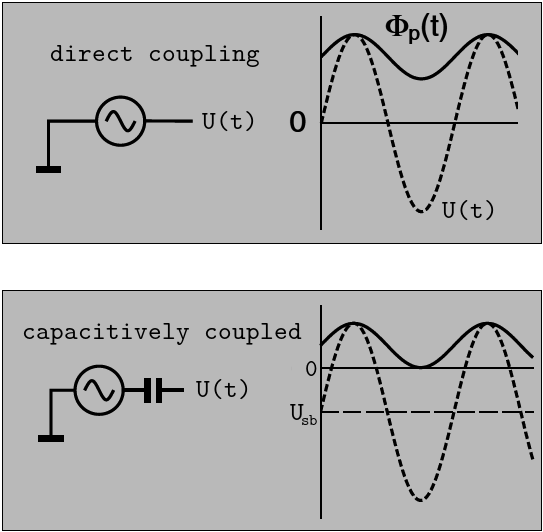
\includegraphics[width=0.95\textwidth]{figures/selfbiasvoltage.png}
					\caption{%
						Schematic course of the voltage $U(t)$ and plasma potential $\Phi(t)$ %
						for a directly and capacitively coupled rf discharge. Different cases of %
						symmetry are shown: enlarged driven electron, grounded %
						electrode and a symmetric discharge.~\cite{Piel10}}\label{fig:circuitselfbias_2}
				\end{figure}
%
				The~\autoref{equ:bulkimpedanz} represents the full electrical impedance, consisting of the inverse sum of real and imaginary resistance, as well as the capacity of the neutral gas volume. Here, $\imag\omega/(\omega\ix{p,e}^{2}C\ix{0})$ characterizes the electrons inertia in regard to an external excitation $\omega$. The real part $\nu\ix{e,n}/(\omega\ix{p,e}^{2}C\ix{0})$ denotes the resistance by neutral particle collisions.
%
				\pagebreak
				\begin{wrapfigure}[16]{r}{0.33\textwidth}
					\centering%
					\vspace*{-0.5cm}%
					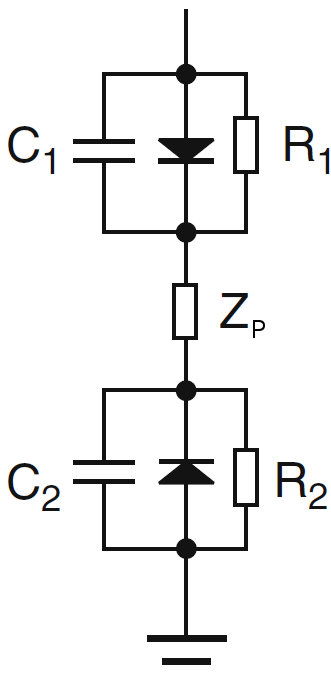
\includegraphics[width=0.22\textwidth]{figures/circuit_selfbias_piel.png}
					\caption{%
						Replacement circuit of an asymmetrically driven ccrf %
						discharge.~\cite{Piel10} A diode represents the directed electron %
						current from the sheaths $j=1,2$.}\label{fig:replacementcurrent}
				\end{wrapfigure}
%
				For high excitation frequencies, e.g.\@ $\SI{13.56}{\mega\hertz}$ the bulk impedance can be neglected (see~\autoref{equ:bulkimpedanz},~\cite{Kay85}). Both sheath capacities of anode and cathode take the dominant part. Therefore, the discharge potential and voltage can be written as:
%
				\begin{align}
					U\left(t\right)=U\ix{sb}+&U\ix{rf}\sin\left(\omega t\right)\,,%
						\nonumber\\[0.0cm]
					&\Phi\ix{p}\left(t\right)=\overline{\Phi\ix{p}}+%
						\Phi\ix{rf}\sin\left(\omega t\right)%
					\label{equ:selfbias_1}
				\end{align}
%
				Both electrodes sheath collapses completely during a full cycle of $U\ix{rf}(t)$, which is why charges can impinge onto the surface and force the plasma potential $\Phi\ix{P}$ to equal out locally with the walls. A short circuit between plasma and sheath occurs when $\Phi\ix{P}$ becomes negative with regard to the excitation. The~\autoref{equ:selfbias_unequal} and~\autoref{fig:circuitselfbias_2} express this circumstance.
%
				\begin{align}
					\Phi\ix{p}\max=\overline{\Phi\ix{p}}+&\Phi\ix{rf}\geq U\ix{sb}+U\ix{rf}\,,%
						\nonumber\\[0.0cm]
					&\Phi\ix{p}\min=\overline{\Phi\ix{p}}-\Phi\ix{rf}\geq0%
						\,\,.%
					\label{equ:selfbias_unequal}
				\end{align}
%     
				If there is no special coupling between electrode and electrical driver, the equality in~\autoref{equ:selfbias_unequal} is true. However, if a capacitive coupling is used, there can't be any net current between excitation and electrode. The capacitance can not be inverted over the course of one rf cycle. The electron currents are then equal on both electrodes, therefore shifting the minimum plasma potential to ground and the maximum to the excitation.
				Finally, the dc \emph{self bias} part $U\ix{sb}$ and the mean plasma potential $\overline{\Phi\ix{p}}$ are
%
				\begin{align}
					\overline{\Phi\ix{p}}=\frac{1}{2}\left(U\ix{sb}+U\ix{rf}\right)\,,%
						\quad\quad%
						U\ix{sb}=\frac{C\ix{1}-C\ix{2}}{C\ix{1}+C\ix{2}}U\ix{rf}%
						\,\,.%
					\label{eq:selfbiaszwei} 
				\end{align}
%
				If the excitation frequency $\omega$ is small compared to other time scales, e.g\@ electron and ion plasma frequencies, the electron current from the sheath $j\ix{L}$ becomes bigger than the displacement current $j\ix{dc}$. Hence the electron current onto the driven electrode decreases by a maxwellian factor --- this is a function of the thereon apllied voltage --- compared to the corresponding ion current. Conclusively, the electrodes sheath impedance is bigger than those of the floating walls. Together with~\autoref{equ:selfbias_1} and~\autoref{equ:inequality} the plasma potential $\Phi\ix{p}$ approximately vanishes, requiring only the currents onto the driven electrode to equal out. For small values of $\omega$~\autoref{equ:selfbias_3} yields the \emph{self bias voltage}~\cite{Piel10}. Here, $\mathbf{I}\ix{0}$ denotes the zeroth order modified \emph{Bessel function}.
%      
				\begin{align}
					U\ix{sb}=\frac{k\ix{B}T\ix{e}}{e}\ln%
						\left[\mathbf{I}\ix{0}\left(\frac{eU\ix{rf}}{k\ix{B}T\ix{e}}\right)\right]%
					\label{equ:selfbias_3}
				\end{align}
%     
